\begin{figure}

  \setlength{\unitlength}{\textwidth}
  \begin{picture}(1,0.25)(0,0.8)
  
    % % %90
      \put(0.025,0.81){\includegraphics[width=0.5\unitlength]{./chapter-pi_1_pi_2/FnP/gnuplot/lift_curve_200.eps}}
      \put(0.495,0.81){\includegraphics[width=0.5\unitlength]{./chapter-pi_1_pi_2/FnP/gnuplot/lift_curve_park.eps}}
 	\put(0.02,0.93){ \large $C_y$} 	
% 	\put(0.56,1.02){ $\theta$}
 	
        \put(0.25,0.8){ $\theta$} 	
        \put(0.75,0.8){ $\theta$}
        
        \put(0.117,1.01){(a)}
        \put(0.565,1.01){(b)}
      \end{picture}

  \caption{Lift coefficient, $C_y$, as a function of incidence angle $\theta$, for a static square cross section. (a) Data from simulations at $Re=200$  and (b) data from \cite{Parkinson1964} at $Re=22300$. Points ($\bullet$) are measurements from the simulations. Curves in both plots are 7th-order interpolating polynomials used to interpolate the fluid forcing for the QSS model.}
    \label{fig:lift_curves}
\end{figure}
